\documentclass{standalone}
\usepackage[usenames,dvipsnames]{xcolor}
\usepackage{tikz}
\usetikzlibrary{arrows.meta}


\begin{document}

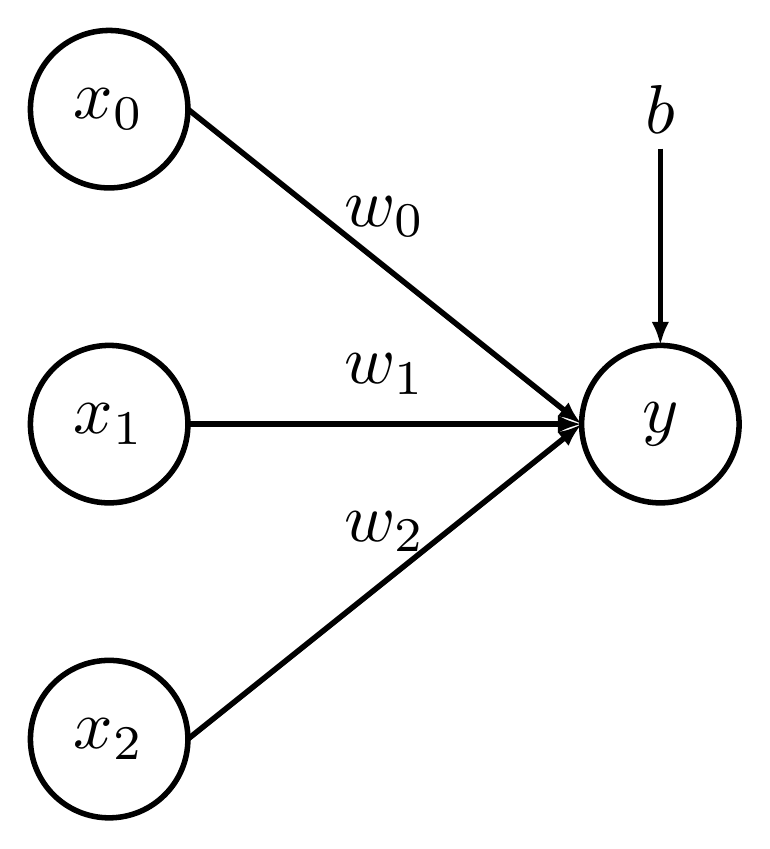
\begin{tikzpicture}

% modify thickness

% input nodes
\draw[line width=2] (-7,4) circle (1cm);
\draw[line width=2] (-7,0) circle (1cm);
\draw[line width=2] (-7,-4) circle (1cm);
\node[scale=2.5] at (-7,4) {$x_0$};
\node[scale=2.5] at (-7,0) {$x_1$};
\node[scale=2.5] at (-7,-4) {$x_2$};

\node[scale=2.5] at (0,4) {$b$};

% output node
\draw[line width=2] (0,0) circle (1cm);
\node[scale=2.5] at (0,0) {$y$};

%\node[draw, circle, scale=2.5, line width=2, minimum size=1cm] (y) at (0,0) {$y$};

% arrows
\draw[line width=2] [-{Latex[length=3mm]}] (-6,4) -- node[above,scale=2.5] {$w_0$} (-1,0);
\draw[line width=2] [-{Latex[length=3mm]}] (-6,0) -- node[above,scale=2.5] {$w_1$} (-1,0);
\draw[line width=2] [-{Latex[length=3mm]}] (-6,-4) -- node[above,scale=2.5] {$w_2$} (-1,0);
\draw[line width=2] [-{Latex[length=3mm]}] (0,3.5) --  (0,1);



\end{tikzpicture}
\end{document}